% xcolor and define colors -------------------------
\usepackage{xcolor}

% https://www.viget.com/articles/color-contrast/
\definecolor{purple}{HTML}{5601A4}
\definecolor{navy}{HTML}{0D3D56}
\definecolor{ruby}{HTML}{9a2515}
\definecolor{alice}{HTML}{107895}
\definecolor{daisy}{HTML}{EBC944}
\definecolor{coral}{HTML}{F26D21}
\definecolor{kelly}{HTML}{829356}
\definecolor{cranberry}{HTML}{E64173}
\definecolor{jet}{HTML}{131516}
\definecolor{asher}{HTML}{555F61}
\definecolor{slate}{HTML}{314F4F}

% Mixtape Sessions
\definecolor{picton-blue}{HTML}{00b7ff}
\definecolor{violet-red}{HTML}{ff3881}
\definecolor{sun}{HTML}{ffaf18}
\definecolor{electric-violet}{HTML}{871EFF}

\newcommand\pictonBlue[1]{{\color{picton-blue}#1}}
\newcommand\sun[1]{{\color{sun}#1}}
\newcommand\electricViolet[1]{{\color{electric-violet}#1}}
\newcommand\violetRed[1]{{\color{violet-red}#1}}

\newcommand\bgPictonBlue[1]{{\colorbox{picton-blue!20!white}{#1}}}
\newcommand\bgSun[1]{{\colorbox{sun!20!white}{#1}}}
\newcommand\bgElectricViolet[1]{{\colorbox{electric-violet!20!white}{#1}}}
\newcommand\bgVioletRed[1]{{\colorbox{violet-red!20!white}{#1}}}

\def\code#1{\texttt{#1}}

% Main theme colors
\definecolor{accent}{HTML}{00b7ff}
\definecolor{accent2}{HTML}{871EFF}
\definecolor{gray100}{HTML}{f3f4f6}
\definecolor{gray800}{HTML}{1F292D}


% Beamer Options -------------------------------------

% Background
\setbeamercolor{background canvas}{bg = white}

% Change text margins
\setbeamersize{text margin left = 15pt, text margin right = 15pt} 

% \alert
\setbeamercolor{alerted text}{fg = accent2}

% Frame title
\setbeamercolor{frametitle}{bg = white, fg = jet}
\setbeamercolor{framesubtitle}{bg = white, fg = accent}
\setbeamerfont{framesubtitle}{size = \small, shape = \itshape}

% Block
\setbeamercolor{block title}{fg = white, bg = accent2}
\setbeamercolor{block body}{fg = gray800, bg = gray100}

% Title page
\setbeamercolor{title}{fg = gray800}
\setbeamercolor{subtitle}{fg = accent}

%% Custom \maketitle and \titlepage
\setbeamertemplate{title page}
{
    %\begin{centering}
        \vspace{20mm}
        {\Large \usebeamerfont{title}\usebeamercolor[fg]{title}\inserttitle}\\
        {\large \itshape \usebeamerfont{subtitle}\usebeamercolor[fg]{subtitle}\insertsubtitle}\\ \vspace{10mm}
        {\insertauthor}\\
        {\color{asher}\small{\insertdate}}\\
    %\end{centering}
}

% Table of Contents
\setbeamercolor{section in toc}{fg = accent!70!jet}
\setbeamercolor{subsection in toc}{fg = jet}

% Button 
\setbeamercolor{button}{bg = accent}

% Remove navigation symbols
\setbeamertemplate{navigation symbols}{}

% Table and Figure captions
\setbeamercolor{caption}{fg=jet!70!white}
\setbeamercolor{caption name}{fg=jet}
\setbeamerfont{caption name}{shape = \itshape}

% Bullet points

%% Fix spacing between items
\let\olditemize=\itemize 
\let\endolditemize=\enditemize 
\renewenvironment{itemize}{\vspace{0.25em}\olditemize \itemsep0.25em}{\endolditemize}

%% Fix left-margins
\settowidth{\leftmargini}{\usebeamertemplate{itemize item}}
\addtolength{\leftmargini}{\labelsep}

%% enumerate item color
\setbeamercolor{enumerate item}{fg = accent}
\setbeamerfont{enumerate item}{size = \small}
\setbeamertemplate{enumerate item}{\insertenumlabel.}

%% itemize
\setbeamercolor{itemize item}{fg = accent!70!white}
\setbeamerfont{itemize item}{size = \small}
\setbeamertemplate{itemize item}[circle]

%% right arrow for subitems
\setbeamercolor{itemize subitem}{fg = accent!60!white}
\setbeamerfont{itemize subitem}{size = \small}
\setbeamertemplate{itemize subitem}{$\rightarrow$}

\setbeamertemplate{itemize subsubitem}[square]
\setbeamercolor{itemize subsubitem}{fg = jet}
\setbeamerfont{itemize subsubitem}{size = \small}








% Links ----------------------------------------------

\usepackage{hyperref}
\hypersetup{
  colorlinks = true,
  linkcolor = accent2,
  filecolor = accent2,
  urlcolor = accent2,
  citecolor = accent2,
}


% Line spacing --------------------------------------
\usepackage{setspace}
\setstretch{1.35}


% \begin{columns} -----------------------------------
\usepackage{multicol}


% Fonts ---------------------------------------------
% Beamer Option to use custom fonts
\usefonttheme{professionalfonts}

% \usepackage[utopia, smallerops, varg]{newtxmath}
% \usepackage{utopia}
\usepackage[sfdefault,light]{roboto}

% Small adjustments to text kerning
\usepackage{microtype}



% Remove annoying over-full box warnings -----------
\vfuzz2pt 
\hfuzz2pt


% Table of Contents with Sections
\setbeamerfont{myTOC}{series=\bfseries, size=\Large}
\AtBeginSection[]{
        \frame{
            \frametitle{Roadmap}
            \tableofcontents[current]   
        }
    }


% Tables -------------------------------------------
% Tables too big
% \begin{adjustbox}{width = 1.2\textwidth, center}
\usepackage{adjustbox}
\usepackage{array}
\usepackage{threeparttable, booktabs, adjustbox}
    
% Fix \input with tables
% \input fails when \\ is at end of external .tex file
\makeatletter
\let\input\@@input
\makeatother

% Tables too narrow
% \begin{tabularx}{\linewidth}{cols}
% col-types: X - center, L - left, R -right
% Relative scale: >{\hsize=.8\hsize}X/L/R
\usepackage{tabularx}
\newcolumntype{L}{>{\raggedright\arraybackslash}X}
\newcolumntype{R}{>{\raggedleft\arraybackslash}X}
\newcolumntype{C}{>{\centering\arraybackslash}X}

% Figures

% \imageframe{img_name} -----------------------------
% from https://github.com/mattjetwell/cousteau
\newcommand{\imageframe}[1]{%
    \begin{frame}[plain]
        \begin{tikzpicture}[remember picture, overlay]
            \node[at = (current page.center), xshift = 0cm] (cover) {%
                \includegraphics[keepaspectratio, width=\paperwidth, height=\paperheight]{#1}
            };
        \end{tikzpicture}
    \end{frame}%
}

% subfigures
\usepackage{subfigure}


% Highlight slide -----------------------------------
% \begin{transitionframe} Text \end{transitionframe}
% from paulgp's beamer tips
\newenvironment{transitionframe}{
    \setbeamercolor{background canvas}{bg=accent!40!black}
    \begin{frame}\color{accent!10!white}\LARGE\centering
}{
    \end{frame}
}


% Table Highlighting --------------------------------
% Create top-left and bottom-right markets in tabular cells with a unique matching id and these commands will outline those cells
\usepackage[beamer,customcolors]{hf-tikz}
\usetikzlibrary{calc}
\usetikzlibrary{fit,shapes.misc}

% To set the hypothesis highlighting boxes red.
\newcommand\marktopleft[1]{%
    \tikz[overlay,remember picture] 
        \node (marker-#1-a) at (0,1.5ex) {};%
}
\newcommand\markbottomright[1]{%
    \tikz[overlay,remember picture] 
        \node (marker-#1-b) at (0,0) {};%
    \tikz[accent!80!jet, ultra thick, overlay, remember picture, inner sep=4pt]
        \node[draw, rectangle, fit=(marker-#1-a.center) (marker-#1-b.center)] {};%
}


% DAGS ----------------------------------------------
\usepackage{tikz}
\usetikzlibrary{shapes,decorations,arrows,calc,arrows.meta,fit,positioning}
% Tikz settings optimized for causal graphs.
\tikzset{
    -Latex,auto,node distance =1 cm and 1 cm,semithick,
    state/.style ={ellipse, draw, minimum width = 0.7 cm},
    point/.style = {circle, draw, inner sep=0.04cm,fill,node contents={}},
    bidirected/.style={Latex-Latex,dashed},
    el/.style = {inner sep=2pt, align=left, sloped}
}


% Beamer tricks -------------------------------------
% Make \pause work in align environments
\makeatletter
\renewrobustcmd{\beamer@@pause}[1][]{%
  \unless\ifmeasuring@%
  \ifblank{#1}%
    {\stepcounter{beamerpauses}}%
    {\setcounter{beamerpauses}{#1}}%
  \onslide<\value{beamerpauses}->\relax%
  \fi%
}
\makeatother


% title page
\title{Nested Logit}
\author{Chris Conlon}
\institute{NYU Stern: Applied Econometrics}

\date{Spring 2023}




\begin{document}



%--------------
% TITLE PAGE
\begin{frame}[plain] %
\titlepage
\end{frame}


\begin{frame}{Reading}
Today's reading is Chapters 4 from:\\
\href{https://eml.berkeley.edu/books/choice2.html}{Ken Train's Discrete Choice Methods with Simulation}
\end{frame}



\begin{frame}
\frametitle{Multinomial Logit: IIA}
The multinomial logit is frequently criticized for producing unrealistic substitution patterns
\begin{itemize}
\item Suppose we got rid of a product $k$ then $s_j^{(1)} = s_j^{(0)} \frac{1}{1- s_k}$.
\item Substitution is just proportional to your pre-existing shares $s_j$
\item No concept of ``closeness'' of competition!
\end{itemize}
\end{frame}

% \begin{frame}
% \frametitle{Can we do better?}
% Multinomial Probit?
% \begin{itemize}
% \item The probit has $\varepsilon_i \sim N(0,\Sigma)$.
% \item If $\Sigma$ is unrestricted, then this can produce relatively flexible substitution patterns.
% \item Flexible is relative: still have normal tails, only pairwise correlations, etc.
% \item It might be that $\rho_{12}$ is large if $1,2$ are similar products.
% \item Much more flexible than Logit
% \end{itemize}
% Downside
% \begin{itemize}
% \item $\Sigma$ has potentially $J^2$ parameters (that is a lot)!
% \item Maybe $J * (J-1)/2$ under symmetry. (still a lot).
% \item Each time we want to compute $s_j(\theta)$ we have to simulate an integral of dimension $J$.
% \item I wouldn't do this for $J \geq 5$.
% \end{itemize}
% \end{frame}

\begin{frame}
\frametitle{Relaxing IIA}
Let's make $\varepsilon_{ij}$ more flexible than IID. Hopefully still have our integrals work out.
\begin{eqnarray*}
u_{ij} =   V_{ij}   + \varepsilon_{ij}
\end{eqnarray*}
\begin{itemize}
\item One approach is to allow for a block structure on $\varepsilon_{ij}$ (and consequently on the elasticities).
\item We assign products into groups $g$ and add a group specific error term
\begin{eqnarray*}
u_{ij} =   V_{ij}  + \eta_{g} + \varepsilon_{ij}
\end{eqnarray*}
\item The trick putting a distribution on $\eta_g + \varepsilon_{ij}$ so that the integrals still work out.
\item Do not try this at home: it turns out the required distribution is known as \alert{GEV} and the resulting model is known as the \alert{nested logit}.
\end{itemize}
\end{frame}

\begin{frame}{Nested Logit}
A traditional (and simple) relaxation of the IIA property is the Nested Logit. This model is often presented as two sequential decisions.
\begin{itemize}
\item First consumers choose a category (following an IIA logit).
\item Within a category consumers make a second decision (following the IIA logit).
\item This leads to a situation where while choices within the same nest follow the IIA property (do not depend on attributes of other alternatives) choices among different nests do not!
\end{itemize}
\end{frame}

\begin{frame}{Alternative Interpretation}
\begin{figure}[htbp]
\begin{center}
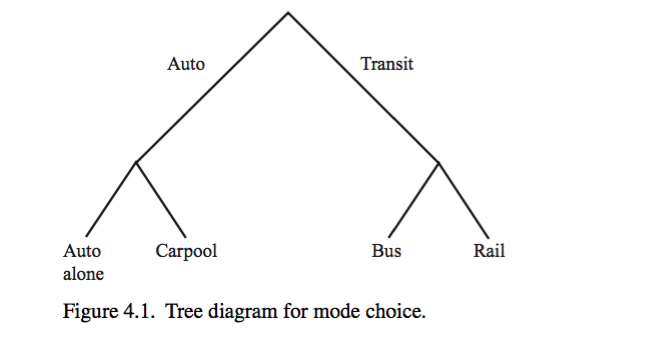
\includegraphics[width=5in]{resources_2/nesting.png}
\end{center}
\end{figure}
\end{frame}

\begin{frame}{Nested Logit}
Utility looks basically the same as before:
\begin{eqnarray*}
U_{ij} = V_{ij} + \underbrace{\eta_{ig} + \widetilde{\varepsilon_{ij}}}_{\varepsilon_{ij}(\lambda_g)}
\end{eqnarray*}
\begin{itemize}
\item We add a new term that depends on the group $g$ but not the product $j$ and think about it as varying unobservably over individuals $i$ just like $\varepsilon_{ij}$.
\item Now $\varepsilon_i \sim F(\varepsilon)$ where $F(\varepsilon) = \exp[-\sum_{g=G}^G \left(\sum_{j \in J_g} \exp[-\varepsilon_{ij}/\lambda_g]\right)^{\lambda_g}$. This is no longer Type I EV but GEV.
\item The key is the addition of the $\lambda_g$ parameters which govern (roughly) the within group correlation.
\item This distribution is a bit cooked up to get a closed form result, but for $\lambda_g \in [0,1]$ for all $g$ it is consistent with random utility maximization.
\end{itemize}
\end{frame}

\begin{frame}{Nested Logit}
\small
The nested logit choice probabilities are:
\begin{eqnarray*}
s_{ij} = \frac{ e^{V_{ij}/\lambda_g} \left(\sum_{k \in J_g} e^{V_{ik}/\lambda_g} \right)^{\lambda_g -1}}{\sum_{h=1}^G \left(\sum_{k \in J_h} e^{V_{ik}/\lambda_h} \right)^{\lambda_h}}
\end{eqnarray*}
Within the same group $g$ we have IIA and proportional substitution 
\begin{eqnarray*}
\frac{s_{ij}}{s_{ik}} = \frac{ e^{V_{ij}/\lambda_g}}{ e^{V_{ik}/\lambda_g}}
\end{eqnarray*}

But for different groups we do not:
\begin{eqnarray*}
s_{ij} = \frac{ e^{V_{ij}/\lambda_g} \left(\sum_{k \in J_g} e^{V_{ik}/\lambda_g} \right)^{\lambda_g -1}}{ e^{V_{ik}/\lambda_h} \left(\sum_{k \in J_h} e^{V_{ik}/\lambda_h} \right)^{\lambda_h -1}}
\end{eqnarray*}
\end{frame}


\begin{frame}{Nested Logit}
We can take the probabilities and re-write them slightly with the substitution that 
$\log \left(\sum_{k \in J_g} e^{V_{ik}} \right)\equiv IV_{ig}$:
\begin{eqnarray*}
s_{ij} &=& \frac{ e^{V_{ij}/\lambda_g}}{ \left(\sum_{k \in J_g} e^{V_{ik}/\lambda_g} \right)}
\cdot
\frac{ \left(\sum_{k \in J_g} e^{V_{ik}/\lambda_g} \right)^{\lambda_g}}{\sum_{h=1}^G \left(\sum_{k \in J_h} e^{V_{ik}/\lambda_h} \right)^{\lambda_h}} \\
&=& \underbrace{\frac{ e^{V_{ij}/\lambda_g}}{ \left(\sum_{k \in J_g} e^{V_{ik}/\lambda_g} \right)}}_{s_{i j | g}}
\cdot
\underbrace{\frac{e^{\lambda_g IV_{ig}}}{\sum_{h=1}^{G} e^{\lambda_h IV_{ih}} }}_{s_{ig}}
\end{eqnarray*}
This is the decomposition into two logits that leads to the ``sequential logit'' story.
\end{frame}

\begin{frame}{Nested Logit : Notes}
\begin{itemize}
\item $\lambda_g=1$ is the simple logit case (IIA)
\item $\lambda_g \rightarrow 0$ implies that all consumers stay within the nest.
\item $\lambda < 0$ or $\lambda > 1$ can happen and usually means something is wrong. These models are not generally consistent with RUM. (If you report one in your paper I will reject it).
\item $\lambda$ is often interpreted as a correlation parameter and this is almost true but not exactly!
\item There are other extensions: overlapping nests, or three level nested logit. 
\item In general the hard part is understanding what the appropriate nesting structure is ex ante. Maybe for some problems this is obvious but for many not.
\end{itemize}
\end{frame}

%\begin{frame}{Nested Logit : Interpretation}
%\begin{itemize}
%\item It is convenient to think about the ``sequential choice'' version of the nested logit.
%\item In practice it is more accurate to think about the structure it imposes on the correlation of $\varepsilon_i$. 
%\item We specify a blocked structure (one block for each nest) and estimate a within vs. across nest correlation parameter.
%\end{itemize}
%\end{frame}


\begin{frame}
\frametitle{Nested Logit}
In practice we end up with the following:
\begin{eqnarray*}
s_{ij} = s_{ij|g}(\theta) s_{ig}(\theta)
\end{eqnarray*}
\vspace{-0.5cm}
\begin{itemize}
\item Because the nested logit can be written as the within group share $s_{ij|g}$ and the share of the group $s_{ig}$ we often explain this model as \alert{sequential choice}
\item First you pick a category, then you pick a product within a category.
\item This is a sometimes helpful (sometimes unhelpful) way to think about this.
\item We can also think about this imposing a block structure on the covariance matrix of $\varepsilon_i$
\item You need to assign products to categories \alert{before you estimate} and you can't make mistakes!
\end{itemize}
\end{frame}

% \begin{frame}
% \frametitle{Nested Logit}
% How does it actually look?
% \begin{eqnarray*}
%  IV_{ig}(\theta) &=& \log \left(\sum_{k \in G} \exp [x_k \beta/(1-\lambda_g)] \right) = E_{\varepsilon}[\max_{j \in G} u_{ij}]\\
%  s_{ij|g}(\theta) &=& \frac{\exp [x_j \beta/(1-\lambda_g)]}{\sum_{k \in G} \exp [x_k \beta/(1-\lambda_g)]} \\
%  s_{ig}(\theta) &=& \frac{\exp [IV_{ig}]^{1-\lambda_g}}{\sum_{h} \exp [IV_{ih}]^{1-\lambda_h}} 
% \end{eqnarray*}
% %\begin{itemize}
% %\item When $\lambda_g \rightarrow 0$ we get the IIA logit model (no correlation within nests)
% %\item When $\lambda_g \rightarrow 1$ we get no across nest substitution.
% %\item When $\lambda_g > 1$ we get something not necessarily consistent with utility maximization!
% %\end{itemize}
% \end{frame}

% \begin{frame}
% \frametitle{Nested Logit}
% How does it actually look?
% \begin{eqnarray*}
% \log \left(\frac{s_{ij|g}(\theta)}{s_{ik|g}(\theta)} \right) = (x_j -x_k)\cdot \frac{\beta}{1-\lambda_g}
%  \end{eqnarray*}
%  \begin{itemize}
% \item We are back to having the IIA property but now within the group $G$.
% \item We also have IIA across groups $g,h$
% \item $\lambda_g$ and $\alpha$ govern the elasticities, which also have a block structure. % expand this later
% \item Sometimes people refer to this as the \alert{product of two logits}
% \item In the old days people used to estimate by fitting sequential IIA logit models -- this is consistent but inefficient -- you shouldn't do this today!
% \item Estimation happens via MLE. This can be tricky because the model is non-convex. It helps to substitute $\tilde{\beta} = \beta/(1-\lambda_g)$
%  \end{itemize}
% \end{frame}

% \begin{frame}
% \frametitle{Parametric Identification}

% Look at derivatives:
% \begin{eqnarray*}
% \frac{\partial\, s_{j|g}}{\partial X_j} &=& \beta_1 s_{j|g}(1-s_{j|g}) \\
%  \frac{\partial\, s_{g}}{\partial X} &=& (1-\lambda) \beta_1 s_{g}(1-s_{g}) \\
%   \frac{\partial\, s_{g}}{\partial J} &=& \frac{1-\lambda}{J} s_{g}(1-s_{g})
% \end{eqnarray*}
% \begin{itemize}
% \item We get $\beta$ by changing $x_j$ within group
% \item We get nesting parameter $\lambda$ by varying $X$
% \item We don't have any parameters left to explain changing number of products $J$.
% \end{itemize}

% \end{frame}



% \begin{frame}
% \frametitle{Nested Logit}
% There are more potential generalizations though they are less frequently used:
%  \begin{itemize}
% \item You can have multiple levels of nesting: first I select a size car (compact, mid-sized, full-sized) then I select a manufacturer, finally a car.
% \item You can have potentially overlapping nests: Yogurt brands are one nest, Yogurt flavors are a second nest. This way strawberry competes with strawberry and/or Dannon substitutes for Dannon.
%  \end{itemize}
% \end{frame}




\section{Convexity and Computation}
\frame{\frametitle{Convexity}
\begin{block}{An optimization problem is convex if}
\begin{eqnarray*}
\min_{x} f(\mathbf{x}) &s.t.& h(\mathbf{x}) \leq 0 \quad A \mathbf{x} = 0
\end{eqnarray*}
\vskip -2ex
\begin{itemize}
\item $f(\mathbf{x}),h(\mathbf{x)}$ are convex (PSD second derivative matrix)
\item Equality Constraint is affine
\end{itemize}
\end{block}
\begin{exampleblock}{Some helpful identities about convexity}
\begin{itemize}
\item Compositions  and sums of convex functions are convex.
\item Norms $||$ are convex, $\max$ is convex, $\log$ is convex
\item  $ \log(\sum_{i=1}^n \exp(x_i))$ is convex.
\item Fixed Points can introduce non-convexities.
\item Globally convex problems have a unique optimum
\end{itemize}
\end{exampleblock}
}

\frame{\frametitle{Properties of Convex Optimization}
\begin{itemize}
\item If a program is globally convex then it has a unique minimizer that will be found by convex optimizers.
\item If a program is not globally convex, but is convex over a region of the parameter space, then most convex optimization routines find any local minima in the convex hull 
\item Convex optimization routines are unlikely to find local minima (including the global minimum) if they do not begin in the same convex hull as the optimum (starting values matter!).
\item Most good commercial routines are clever about dealing with multiple starting values and handling problems that are well approximated by convex functions.
\item Good Routines use information about sparseness of Hessian -- this generally determines speed.
\end{itemize}
}

\subsection{Nested Logit Example}


%\subsection{Logit and Nested Logit}
%\frame{\frametitle{Logit Model}
%Easy to see that FIML estimator is convex:
%\begin{eqnarray*}
%\min_{\theta} \sum_j q_j \ln \left(\frac{\exp[x_j \beta ]}{1+\sum_j \exp[x_j \beta]} \right)\\
%\min_{\theta} \sum_j q_j \left( x_j \beta  - \ln \left(1+\sum_j \exp[x_j \beta ]\right) \right)\\
%\end{eqnarray*}
%}

\begin{frame}{Nested Logit Model}
\begin{exampleblock}{FIML Nested Logit Model is Non-Convex}
\begin{eqnarray*}
\min_{\theta} \sum_j q_j \ln S_j(\theta) \quad \mbox{s.t.} \quad  S_j(\theta) = \frac{e^{x_j \beta/ \lambda}( \sum_{k \in g_l} e^{x_j \beta/ \lambda})^{\lambda-1}}{\sum_{\forall l'} ( \sum_{k \in g_l'} e^{x_j \beta/ \lambda})^{\lambda} }
\end{eqnarray*}
This is a pain to show but the problem is with the cross term $\frac{\partial^2 S_j}{\partial \beta \partial \lambda}$ because $\exp[x_j \beta / \lambda]$ is not convex.
\end{exampleblock}
\begin{exampleblock}{A Simple Substitution Saves the Day:  let $\gamma = \beta / \lambda$}
\begin{eqnarray*}
\min_{\theta} \sum_j q_j \ln S_j(\theta) \quad \mbox{s.t.} \quad  
S_j(\theta) = \frac{e^{x_j \gamma}( \sum_{k \in g_l} e^{x_j \gamma})^{\lambda-1}}{\sum_{\forall l'} ( \sum_{k \in g_l'} e^{x_j \gamma})^{\lambda} }
\end{eqnarray*}
This is much better behaved and easier to optimize.
\end{exampleblock}
\end{frame}

\begin{frame}{Nested Logit Model}
\begin{center}
\begin{tabular}{lrrr}
&\bf{Original} & \bf{Substitution} & \bf{No Derivatives} \\
Parameters &49& 49&49\\
Nonlinear $\lambda$ &5 &5 &5\\
Likelihood & 2.279448 &2.279448  & 2.27972\\
Iterations &197 &146 & 352\\
Time & 59.0 s & 10.7 s & 192s  \\
\end{tabular}
\end{center}
Discuss Nelder-Meade
\end{frame}

\begin{frame}{Computing Derivatives}
A key aspect of any optimization problem is going to be computing the derivatives (first and second) of the model.  There are some different approaches
\begin{itemize}
\item Numerical: Often inaccurate and error prone (why?) $f'(x) \approx \frac{f(x+h)-f(x-h)}{2h}$
\item Pencil and Paper: this tends to be mistake prone -- but often actually the fastest
\item Automatic: Software brute forces through a chain rule calculation at every step (limited language). See \texttt{jax} in \texttt{Python} or \texttt{Optimization.jl} in \texttt{Julia}.
\item Symbolic (Maple/Mathematica): software ``knows'' derivatives of certain objects and can do its own simplification.  (limited language).
\end{itemize}
\end{frame}






\section*{Thanks}
\end{document}

